\documentclass[aps,prl,reprint]{revtex4-1}
\usepackage[utf8]{inputenc}
\usepackage{gensymb}
\usepackage{float}
\usepackage[spanish]{babel}
\usepackage{graphicx}
\usepackage{babel}
\usepackage{amsmath}
\begin{document}
\title{Laboratorio Microondas}

\author{Daniel Fajardo}
\author{Juan Sebastian Vargas}
\affiliation{Universidad de los Andes, Departamento de f\'isica}
 

\date{18 de febrero de 2016}

\setlength{\columnsep}{1cm}





\begin{abstract}
    
La radiación electromagnética, que esta compuesta por ondas electromagnéticas, fue descubierta en los inicios del siglo 19. Las Microondas son ampliamente utilizadas en telecomunicaciones, radares y muchos usos mas. En este experimento se utilizo un emisor de microondas con $\lambda= 2.85 cm$ con el cual se observaron varios fenómenos de las ondas E.M.\\
\textit{Palabras clave: Radiación Electromagn\'etica, Microondas, Campos El\'ectrico, Campo Magnetico, Polarización}


\end{abstract}
\maketitle

\section{Introducci\'on}
    SE DEBE HACER UN MARCO TEORICO DE:
    ONDAS ELECTROMAGNETICAS, POLARIZACION, RESULTADOS ESPERADOS DE LOS EXPERIMENTOS, angulo de brewster \\
//La Polarizacion es un vector que apunta en la misma //dirección que  $\vec{E}$: $\vec{n}$

\section{Montaje Experimental}

El primer montaje consiste colocar el emisor frente al recibidor, y variar la distancia entre los dos como se muestra en la figura \ref{monta1}:\\
\begin{figure}[H]
\begin{center}
 \scalebox{0.4}{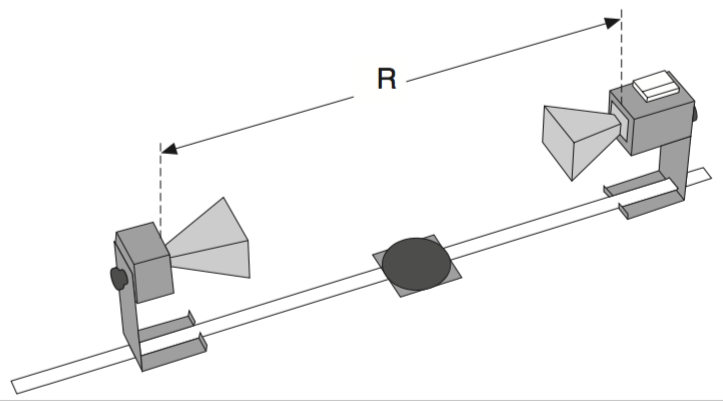
\includegraphics{monta1.png}} 
 \caption{Primer montaje}
 \label{monta1}
 \end{center}
\end{figure}


Donde se varia la distancia $R$ y se anota su respectivo valor de intensidad dado por el recibidor. Se hizo la medición para 7 diferentes valores de $R$ con valores entre $40 cm$ hasta $100 cm$. \\


El segundo montaje consiste colocar el emisor y el recibidor en el goniometro, y variar el ángulo y medir como cambia la lectura del recibidor a medida que cambiamos el ángulo entre los dos como se muestra en la figura \ref{monta2}:\\
\begin{figure}[H]
\begin{center}
 \scalebox{0.4}{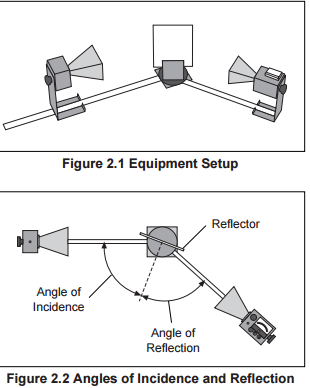
\includegraphics{Montaje 2.png}} 
 \caption{Segundo montaje}
 \label{monta2}
 \end{center}
\end{figure}

Para el tercer montaje tenemos una configuración similar a la Figura 1 pero esta vez mediremos la longitud de la onda que genera el emisor. Se pondrá el Emisor y recibidor a una distancia tal que este en un máximo de intensidad, se anota la distancia entre los equipos, luego se alejan mientras se cuentan al menos 10 mínimos, y se coloca en el siguiente máximo  volviendo a medir la distancia entre los equipos. Con estos datos es posible medir la longitud de onda.
\\

Para el cuarto montaje se dispondrá de un montaje similar al de la Figura 1, sólo que esta vez se interpondrá un objeto que para los objetivos de este experimento hará las veces de prisma y mostrará la ley de Snell.Lo que se hará será variar el ángulo y encontrar el máximo. El montaje es como se muestra e la figura:
\ref{monta2}:\\
\begin{figure}[H]
\begin{center}
 \scalebox{0.4}{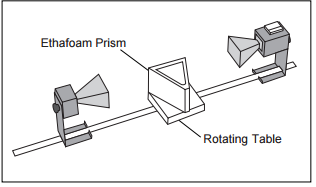
\includegraphics{Montaje 4.png}} 
 \caption{Cuarto montaje}
 \label{monta3}
 \end{center}
\end{figure}

Para el quinto montaje se volvi\'o a utilizar el de la Figura 1 dejando un $R$ constante,  se rot\'o el recibidor cada $10\degree$ empezando en su posición natural ($0\degree$) hasta $180\degree$.

\begin{figure}[H]
\begin{center}
 \scalebox{0.7}{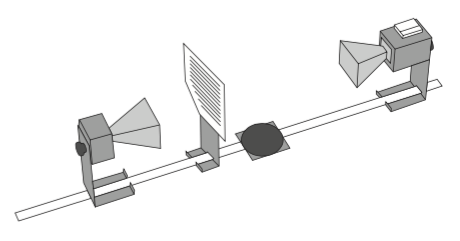
\includegraphics{exp5.png}} 
 \caption{Variaci\'on quinto montaje}
 \label{exp5}
 \end{center}
\end{figure}

Para la segunda parte de este quinto experimento se coloc\'o un material reflector con rendijas en la mitad del emisor y recibidor tal y como se muestra en la Figura \ref{exp5}. Se rot\'oe el emisor y se anoto la intensidad mostrada por el recibidor\\

Para el sexto montajese hará interferencia con doble rendija y se medira la intensidad para distintos ángulos y con ello hallar la longitud de onda como se muestra en la figura: \begin{figure}[H]
\begin{center}
 \scalebox{0.7}{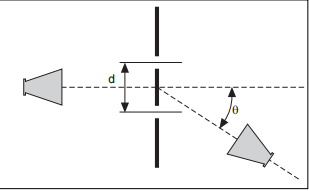
\includegraphics{Montaje 6.png}} 
 \caption{Variaci\'on sexto montaje}
 \label{exp6}
 \end{center}
\end{figure}
\\

Para este séptimo montaje se pusieron el emisor y recibidor de frente, en la mitad se coloco un reflector, como se muestra en la Figura \ref{exp5}, moviendo el reflector se busco un mínimo y en este punto se miden la distancia entre emisor y recibidor, y la distancia a la que se encuentra el reflector, luego se aleja el reflector hasta encontrar nuevamente un mínimo, se vuelven a tomar los datos. Con estos datos es posible calcular la longitud de onda $\lambda$ así:

\begin{equation*}
    \lambda=|L_{1}-L_{2}|
\end{equation*}
\begin{equation*}
    L_{n}=2\sqrt{d^{2}+h_{n}^{2}}
\end{equation*}

Donde $L_{n}$ es la longitud del camino que recorre la onda reflejada, $d$ es la mitad de la separación que hay entre emisor-recibidor y $h_{n}$ es la distancia a la que se encuentra el reflector para ese camino.


\begin{figure}[H]
\begin{center}
 \scalebox{0.7}{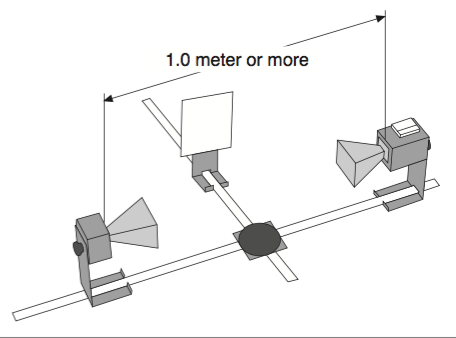
\includegraphics{exp7.png}} 
 \caption{S\'eptimo montaje}
 \label{exp7}
 \end{center}
\end{figure}

\\
En este experimento se hará un interferometro de Fabry-Perot que consiste en un montaje similar al de la figura 1 sólo que se interpondran dos reflectores parciales en el camino, se medirá minimos y maximos al variar la distancia entre los reflectores parciales.

\\

En este noveno montaje se intentara recrear el interferómetro de Michelson, el montaje consta de dos reflectores A y B, además de un reflector parcial C, tal y como se muestra en la Figura \ref{exp9}. Se moverá el reflector A y de esta manera generar cambios en las lecturas, estos máximos y m\'inimos son la evidencia de que las ondas desviadas están en fase con las que no se desviaron y as\'i lograr volver a medir la longitud de onda $\lambda$.

\begin{figure}[H]
\begin{center}
 \scalebox{0.7}{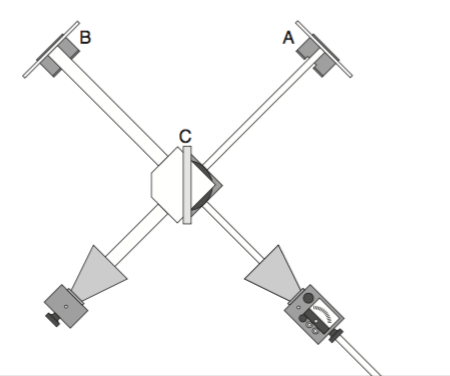
\includegraphics{exp9.png}} 
 \caption{Noveno montaje}
 \label{exp9}
 \end{center}
\end{figure}
\\
En el décimo montaje se hará una fibra óptica con una bolsas tubulares llenas de bolitas de estireno que funcionaran como el medio con indice de refracción mayor y permitirán la reflexión total interna que caracteriza la fibra óptica.

\\
En este montaje se buscara encontrar evidencia del ángulo de Brewster para el montaje será como en la Figura \ref{exp11}. Se pondrá el panel de polietileno de tal manera que el ángulo de incidencia de las microondas sea $20\degree$, y luego tomar las lecturas de la intensidad para 12 diferentes ángulos .


\begin{figure}[H]
\begin{center}
 \scalebox{0.7}{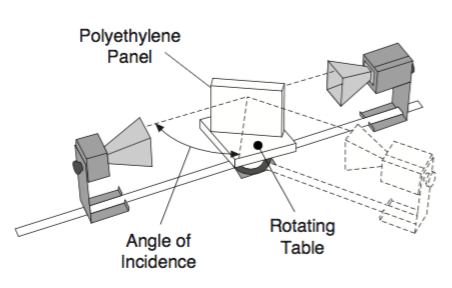
\includegraphics{exp11.png}} 
 \caption{Montaje 11}
 \label{exp11}
 \end{center}
\end{figure}

\section{Resultados y An\'alisis}
En la Tabla \ref{tbmonta1.1} podemos ver la relación entre la distancia $R$ y la intensidad relativa medida por el recibidor:\\

\begin{table}[H]
\begin{center}

\begin{tabular}{|| r || c ||} 
\hline\hline
R$\pm$ 0.1(cm)  & Medicion $\pm$ 0.02 (mA) \\ \hline
40             & \textgreater 1        \\ \hline
50             & 0.86              \\ \hline
60             & 0.65              \\ \hline
70             & 0.50              \\ \hline
80             & 0.36              \\ \hline
90             & 0.2               \\ \hline
100            & 0.14              \\ \hline

\end{tabular}
\end{center}
\caption{Tabla que muestra la medicion con su respectivo valor de R}
\label{tbmonta1.1}
\end{table}


\begin{figure}[H]
 \scalebox{0.5}{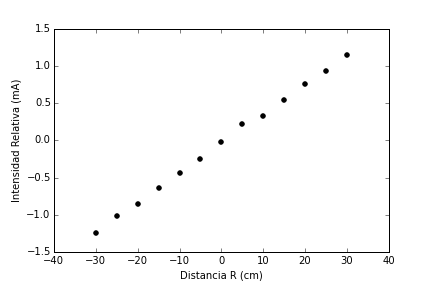
\includegraphics{grmonta1_1.png}} 
 \caption{Grafico de la intensidad contra distancia}
 \label{gmonta1.1}
\end{figure}


En la Figura \ref{gmonta1.1} vemos una grafica de los puntos de la Tabla \ref{tbmonta1.1} y a simple vista se puede ver que la intensidad medida es inversamente proporcional a la distancia, resultado que no nos sorprende ya que la intensidad disminuye con la distancia.\\



En la Tabla \ref{tbmonta2} podemos ver la relación entre el ángulo de incidencia y el ángulo de reflexión es decir donde la medida es máxima y donde la teoria predice que es la misma:\\

\begin{table}[H]
\begin{center}

\begin{tabular}{|| r || c ||} 
\hline\hline
\'Angulo Incidencia$\pm$ 1(\degree)  & \'A Reflexi\'on $\pm$ 1 (\degree) \\ \hline
20             & 16        \\ \hline
30             & 26              \\ \hline
40             & 44              \\ \hline
50             & 55              \\ \hline
60              & 62              \\ \hline
70 & 62 \\ \hline
80             & 72               \\ \hline
90            & 68              \\ \hline

\end{tabular}
\end{center}
\caption{Tabla que muestra la medicion con su respectivo valor de R}
\label{tbmonta2}
\end{table}

Los datos reflejan lo que la teoría predice con un error en promedio del 14 porciento. Lo cual es suficiente cercano para rectificar la teoría de la reflexión.

Con el tercer montaje buscábamos medir la longitud de onda $\lambda$, nuestra distancia inicial fue $44 \pm 0.1 \text{cm}$ y luego de contar 10 m\'inimos se encontró el siguiente máximo a $58.5 \pm 0.1 \text{cm}$. lo que nos deja la distancia recorrida como $\Delta R= 14.5\pm 0.1 \text{cm}$.Para calcular $\lambda$ utilizamos:
\begin{equation}\label{longitudOnda}
    \Delta R=\frac{n\lambda}{2}
\end{equation}

Donde $n$ es el numero de minimos atravesados. Obtuvimos el resultado:
\begin{equation*}
\lambda=2.9\pm 0.02 \text{cm} 
\end{equation*}
Este resultado es muy cercano a el valor teórico que es de $2.85 \text{cm}$ .\\
En este experimento la idea es comprobar la ley de snell que es la siguiente:
\begin{equation}\label{leysnell}
    n_1 sen(\theta_1)= n_2 sen( \theta_2)
\end{equation} 
En este caso el angulo \begin{equation}\label{angulo1}
    \theta_1=90\pm 1\degree
\end{equation} \\  por lo que el seno vale uno y la ecuación se reduce a la siguiente:

\begin{equation}\label{leysnellsimplificada}
    n_1 = n_2 sen( \theta_2)
\end{equation} 
En este caso \begin{equation}\label{angulo}
    \theta_2=78\pm 1\degree
\end{equation} \ entonces si reemplazamos obtendriamos que el indice de refracción del estireno sabiendo que el de aire es 1 sería \begin{equation}\label{angulo}
    n_2=1.90 \pm 0.02
\end{equation}\\ Si comparamos con los datos reales obtendriamos un error aproximado del 20 porciento pues el valor real es 1.5.

Cuando dejamos $R$ constante y rotamos el recibidor en el quinto montaje obtenemos la siguiente tabla:

\begin{table}[H]
\begin{center}

\begin{tabular}{|| r || c ||} 
\hline\hline
Angulo Recibidor$\pm$ 1(\degree) & Medicion$\pm$ 0.02 (mA) \\ \hline
0             & 1        \\ \hline
10             & 1              \\ \hline
20             & 0.95              \\ \hline
30             & 0.84              \\ \hline
40             & 0.70              \\ \hline
50             & 0.52              \\ \hline
60            & 0.28             \\ \hline
70 & 0.07 \\ \hline
80 & 0 \\ \hline
90 & 0 \\\hline
100 & 0 \\ \hline
110 & 0 \\ \hline
120 & 0.04 \\ \hline
130 & 0.37 \\ \hline
140 & 0.58 \\ \hline
150 & 0.77 \\ \hline
160 & 0.92 \\ \hline
170 & 1 \\ \hline
180 & \textgreater 1 \\ \hline

\end{tabular}
\end{center}
\caption{Tabla de la variacion de la Intensidad en funci\'on del angulo}
\label{tbmonta1.2}
\end{table}
Graficando los puntos de la Tabla \ref{tbmonta1.2}:

\begin{figure}[H]
 \scalebox{0.5}{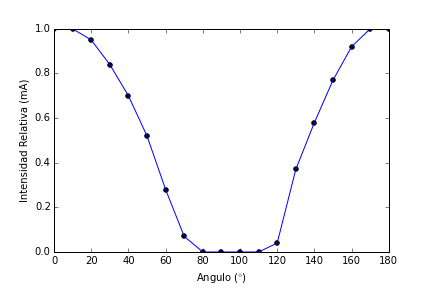
\includegraphics{grmonta1_2.png}} 
 \caption{Grafico de Intensidad contra Angulo de rotacion}
 \label{gmonta1.2}
\end{figure}
En la Figura \ref{gmonta1.2} obtenemos un resultado esperado, ya que el emisor genera ondas que tienen polarización lineal, cuando el vector $\vec{n}$ se encuentra en la misma dirección que el diodo detector ($\theta=0\degree$) la intensidad será máxima, ya que las polarizaciones coincides, cuando este ángulo va cambiando la intensidad disminuye, hasta el punto en el que la Intensidad es mínima cuando $\vec{n}$ es perpendicular a el diodo detector ($\theta=90\degree$). Esto rectifica la ley de Malus que predice que la intensidad es proporcional al cuadrado del coseno que forman la polarización con la onda.

\begin{figure}[H]
\begin{center}
 \scalebox{0.7}{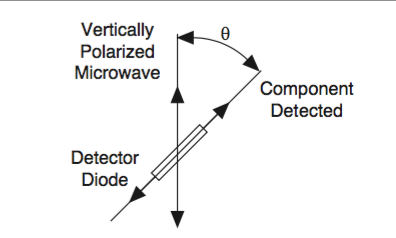
\includegraphics{polari.png}} 
 \caption{Dirección de la polarización y del diodo detector}
 \label{polari}
 \end{center}
\end{figure}

Para la segunda parte de este quinto experimento se gener\'o esta tabla:


\begin{table}[H]
\begin{center}

\begin{tabular}{|| r || c ||} 
\hline\hline
\'Angulo del emisor$\pm$ 1(\degree)  & Medicion $\pm$ 0.02 (mA) \\ \hline
0             & 0.90        \\ \hline
22.5             & 0.13             \\ \hline
45            & 0.01             \\ \hline
67.5             & 0              \\ \hline
90             & 0             \\ \hline


\end{tabular}
\end{center}
\caption{Resultados segundo montaje}
\label{tbexp5}
\end{table}
Como vemos el polarizador bloquea la onda cuando la polarización de esta es perpendicular a la dirección de las ranuras($90\degree$) .

En este experimento se quiere comprobar la teoria de la interferencia de doble rendija sabiendo lo siguiente:
\begin{equation*}
    \lambda = 2.85 \text{cm}
\end{equation*}
Hay máximos cuando:
\begin{equation*}
    d sin(\theta) = n \lambda
\end{equation*}
La separación de las rendijas es:
\begin{equation*}
    d = 9.00\pm 0.05 \text{cm}
\end{equation*}
La comparación de los máximos medidos y los máximos que predicen la teoria difieren aproximadamente en un 10 porciento.
\begin{table}[H]
\begin{center}

\begin{tabular}{|| r || c ||} 
\hline\hline
\'Angulo $\pm$ 1(\degree)  & Medicion $\pm$ 0.02 (mA) \\ \hline
0             & 0.06        \\ \hline
5             & 0.04              \\ \hline
10             & 0.01              \\ \hline
15             & 0.11              \\ \hline
20             & 0.10              \\ \hline
25             & 0.01              \\ \hline
30            & 0.03             \\ \hline
35 & 0.07 \\ \hline
40 & 0.03 \\ \hline
45 & 0.01 \\ \hline
50 & 0.02 \\ \hline
55 & 0.04 \\ \hline
60 & 0.04 \\ \hline
65 & 0.03 \\ \hline
70 & 0.02 \\ \hline
75 & 0.02 \\ \hline
80 & 0.015 \\ \hline
85 & 0.01 \\ \hline


\end{tabular}
\end{center}
\caption{Relacion \'angulo y intensidad del sexto montaje}
\label{tbmonta6}
\end{table}

\begin{figure}[H]
\begin{center}
 \scalebox{0.5}{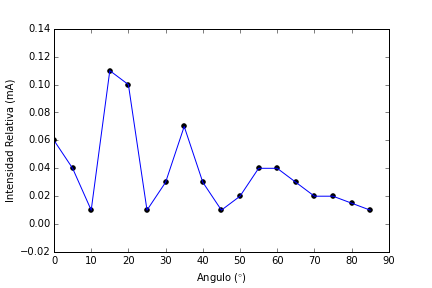
\includegraphics{grmonta6.png}} 
 \caption{Grafica doble rendija, sexto montaje}
 \label{grmonta6}
 \end{center}
\end{figure}

Para el séptimo montaje se tomaron dos grupos de datos, para el primer intento se encontró que $h_1=13.0\pm 0.1 \text{cm}$, $h_2=18.4\pm 0.1 \text{cm}$ y $d=52.4\pm 0.1 \text{cm}$. Para el segundo intento se obtuvo que $h_1=12.4\pm 0.1 \text{cm}$, $h_2=17,5\pm 0.1 \text{cm}$ y $d=55.1\pm 0.1 \text{cm}$. Los valores obtenidos para $\lambda$ son:
\begin{equation*}
    \lambda_1 = 3.1 \pm 0.5 \text{cm}
\end{equation*}
\begin{equation*}
    \lambda_2 = 2.8 \pm 0.5 \text{cm}
\end{equation*}
Podemos ver que el segundo intento fue mucho mas cercano al valor teórico, pero aun así el primer intento es un valor muy cercano también lo cual nos indica que este método es efectivo para medir la longitud de onda.

\\
 En el octavo experimento se comprueba la longitud de onda mediante la interferencia sabiendo que la ecuación que describe los minimos es
 \begin{equation*}
    \Delta L = n \lambda /2
    \end{equation*}
    Se tomó un minimo y se midio la distancia de separación y luego se movio hasta que pasaron 10 máximos y se midio la distancia del nuevo minimo se hizo esto dos veces.
    $d_1=23,5\pm 0.1 \text{cm}$ y 10 minimos después $d_1=38,0\pm 0.1 \text{cm}$  lo que implica que $-\lambda = 2,80\pm 0.01 \text{cm}$ se repitió el proceso para $d_3=32,0\pm 0.1 \text{cm}$ y diez minimos después $d_4=46,4\pm 0.1 \text{cm}$ lo que da: $\lambda =2.88\pm 0.01 \text{cm}$ lo que da en promedio: \begin{equation*}
    \ \lambda =2.84\pm 0.01
    \end{equation*}
    Lo cual es extremedamente cercano a lo que dice la teoría con un error inferior al uno porciento.

 
 
\textbf{RESULT 9}\\
En el décimo experimento se uso una fibra óptica con bolas de estireno y se rectificó que con la fibra óptica la lectura es mayor que sin nada entre el recibidor y el emisor, también se comprobó que cuando la fibra óptica está recta se obtiene un máximo en la lectura y a medida que se dobla esta lectura disminuye\\

\begin{table}[H]
\begin{center}

\begin{tabular}{|| r || c || r ||} 
\hline\hline
\'Angulo $\pm$ 1(\degree) &
\begin{tabular}[c]{@{}l@{}}M Horizontal   \\ $\pm$ 0.02 (mA) \end{tabular}&
\begin{tabular}[c]{@{}l@{}}M Vertical   \\ $\pm$ 0.02 (mA) \end{tabular} \\ \hline
20 & 1 & 0.8 \\ \hline
25 & 0.76  &    0.9         \\ \hline
30            & 0.32 & 0.7             \\ \hline
35 & 0.04 & 0.4 \\ \hline
40 & 0.0 & 0.1 \\ \hline
45 & 0.0 & 0.02 \\ \hline
50 & 0.0 & 0.0 \\ \hline
55 & 0.0 & 0.0 \\ \hline
60 & 0.0 & 0.0 \\ \hline
65 & 0.0 & 0.0 \\ \hline
70 & 0.0 & 0.0 \\ \hline
75 & 0.0 & 0.0 \\ \hline
80 & 0.0 & 0.0 \\ \hline
85 & 0.0 & 0.0 \\ \hline


\end{tabular}
\end{center}
\caption{Tabla resultados \'angulo Brewster}
\label{tbmonta11}
\end{table}


\begin{figure}[H]
\begin{center}
 \scalebox{0.5}{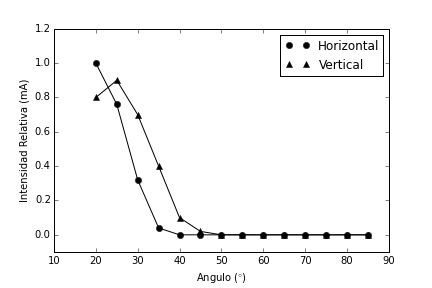
\includegraphics{grmonta11.png}} 
 \caption{\'Angulo Brewster}
 \label{grmonta11}
 \end{center}
\end{figure}

\section{Conclusiones}
Durante el experimento se comprobaron varios principios de la óptica como la intensidad que disminuye con la distancia de manera inversamente proporcional, también la ley de malus que implica que la intensidad disminuye como el coseno cuadrado del ángulo de polarización. 
También se comprobó que el angulo de reflexión es aproximadamente el mismo que el ángulo de incidencia. Se halló en varias ocasiones la longitud de onda usada en el experimento con una exactitud hasta menor al uno porciento.
Por otro lado se verificó la teoria detrás dde la interferencia por doble rendija.

\end{document}
